\documentclass{book}
\usepackage{fullpage}
\usepackage{graphicx}
\title{Project Two \\Neural Networks \\ Writeup}
\author{Ben Cohen}
\begin{document}
\maketitle
\section*{Network Design}
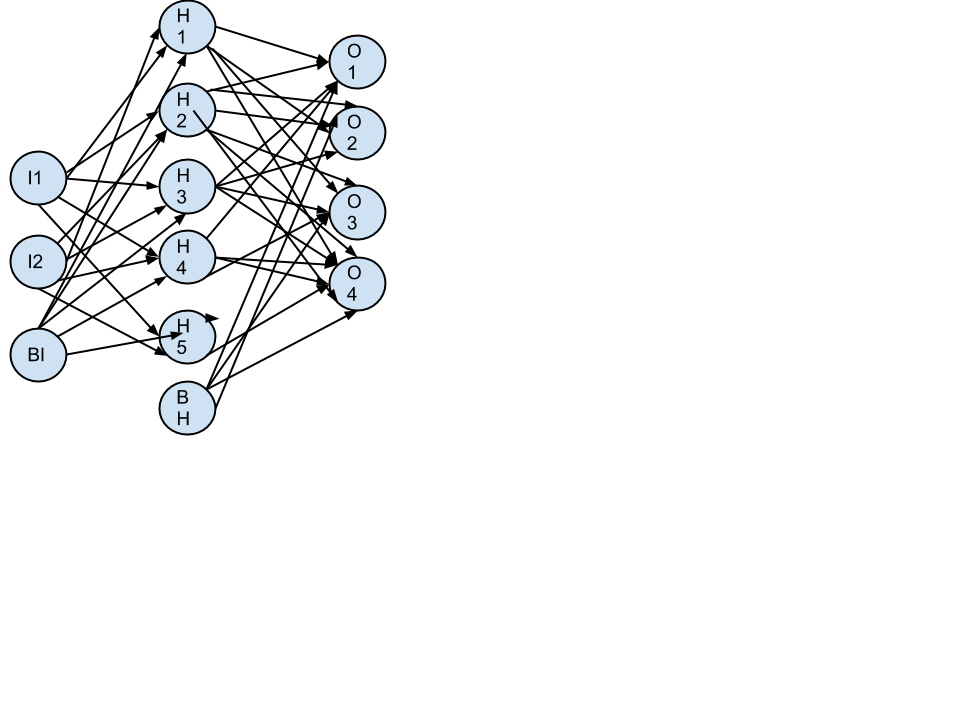
\includegraphics[scale=0.5]{arch.png}
\indent I used a 2-5-4 architecture as was specified in the assignment.  This architecture has a fairly limited set of functions that it can represent, and this class is pretty severely limited by the number if input nodes.  Most problems that have any level of complexity require more input nodes, and probably more hidden nodes.  That being said, I think this architecture was pretty well suited to this problem, and I got pretty good results in good time, so it served it's purpose.  I also thought that since there were not too many hidden nodes, there would be less overfitting as the network doesn't have the space to learn really specific things.  I think my hypothesis was correct, as I didn't see much overfitting at all.  With a few bumps I had a constant decrese in my error as I ran more and more epochs.  
\section*{Data Sets}
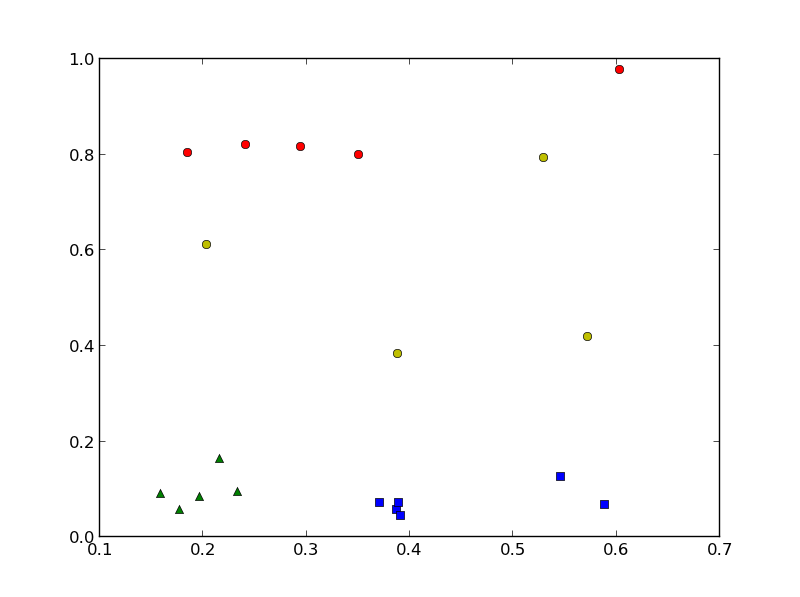
\includegraphics[scale=0.45]{function.png}
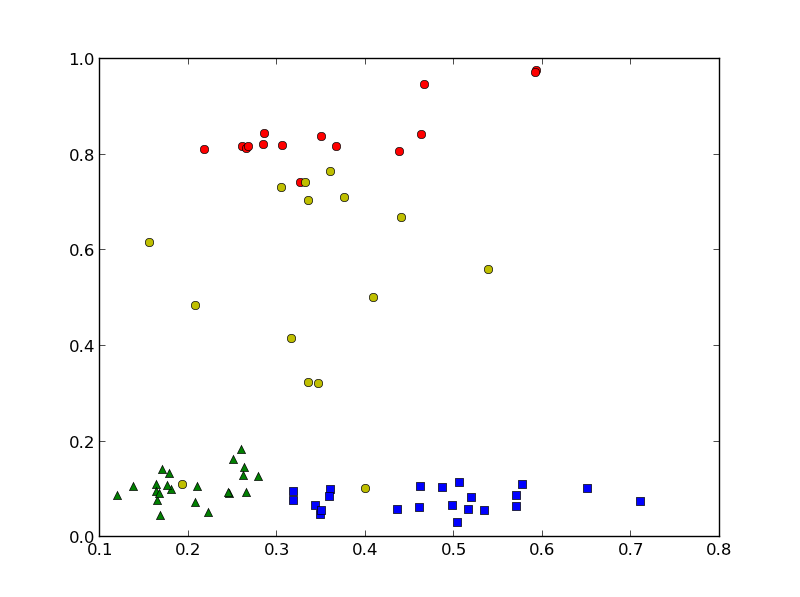
\includegraphics[scale=0.45]{training.png}
The above chart on the left is the test data, and the above chart on the right is the training data.  These sets have an interesting distribution.  The training set has a lot of noise.  In particular, there is one yellow (scrap) dot in the general region of each of the other classes.  I'm sure this noise threw off the data a bit, but in general my network still learned the function rather well.  The test data was much less noisy, and I was unsurprisingly got better results on it (~85 - ~90 vs ~75 to ~85 on training data).  Additionally, I was able to hit 100 percent accuracy with another network architecture that was able to better compensate for the noise.  
\section*{Results}
Test Data
\\
0 epochs
\\
===============
\\
   B  N  R  S
\\
B [5, 6, 5, 4]
\\
N [0, 0, 0, 0]
\\
R [0, 0, 0, 0]
\\
S [0, 0, 0, 0]
\\
Profit: -0.05
\\
We got 5 out of 20 correct for an accuracy of: 0.25 percent on the test data.
\\
10 epochs
\\
===============
\\
   B  N  R  S
\\
B [0, 0, 0, 0]
\\
N [0, 0, 0, 0]
\\
R [5, 6, 5, 4]
\\
S [0, 0, 0, 0]
\\
Profit: -0.8
\\
We got 5 out of 20 correct for an accuracy of: 0.25 percent on the test data.
\\
100 epochs
\\
===============
\\
   B  N  R  S
\\
B [0, 0, 0, 0]
\\
N [0, 0, 0, 0]
\\
R [5, 6, 5, 4]
\\
S [0, 0, 0, 0]
\\
Profit: -0.8
\\
We got 5 out of 20 correct for an accuracy of: 0.25 percent on the test data.
\\
1000 epochs
\\
===============
\\
   B  N  R  S
\\
B [5, 0, 0, 1]
\\
N [0, 6, 0, 0]
\\
R [0, 0, 5, 2]
\\
S [0, 0, 0, 1]
\\
Profit: 1.91
\\
We got 17 out of 20 correct for an accuracy of: 0.85 percent on the test data.
\\
10000 epochs
\\
===============
\\
   B  N  R  S
\\
B [4, 0, 0, 0]
\\
N [0, 6, 0, 0]
\\
R [0, 0, 5, 2]
\\
S [1, 0, 0, 2]
\\
Profit: 1.72
\\
We got 17 out of 20 correct for an accuracy of: 0.85 percent on the test data.\\\\\\
Training Data
\\
0 epochs
\\
===============
\\
   B  N  R  S
\\
B [15, 22, 22, 15]
\\
N [0, 0, 0, 0]
\\
R [0, 0, 0, 0]
\\
S [0, 0, 0, 0]
\\
Profit: -1.13
\\
We got 15 out of 74 correct for an accuracy of: 0.202702702703 percent on the training data.
\\
10 epochs
\\
===============
\\
   B  N  R  S
\\
B [0, 0, 0, 0]
\\
N [0, 0, 0, 0]
\\
R [15, 22, 22, 15]
\\
S [0, 0, 0, 0]
\\
Profit: -2.54
\\
We got 22 out of 74 correct for an accuracy of: 0.297297297297 percent on the training data.
\\
100 epochs
\\
===============
\\
   B  N  R  S
\\
B [0, 0, 0, 0]
\\
N [0, 0, 0, 0]
\\
R [15, 22, 22, 15]
\\
S [0, 0, 0, 0]
\\
Profit: -2.54
\\
We got 22 out of 74 correct for an accuracy of: 0.297297297297 percent on the training data.
\\
1000 epochs
\\
===============
\\
   B  N  R  S
\\
B [15, 0, 0, 6]
\\
N [0, 22, 0, 1]
\\
R [0, 0, 22, 6]
\\
S [0, 0, 0, 2]
\\
Profit: 6.43
\\
We got 61 out of 74 correct for an accuracy of: 0.824324324324 percent on the training data.
\\
10000 epochs
\\
===============
\\
   B  N  R  S
\\
B [11, 0, 0, 4]
\\
N [0, 22, 0, 1]
\\
R [0, 0, 22, 3]
\\
S [4, 0, 0, 7]
\\
Profit: 5.71
\\
We got 62 out of 74 correct for an accuracy of: 0.837837837838 percent on the training data.\\
\section*{Regions}
\hspace{50px}0 Epochs \hspace{80px}10 Epochs \hspace{100px}100 Epochs \\
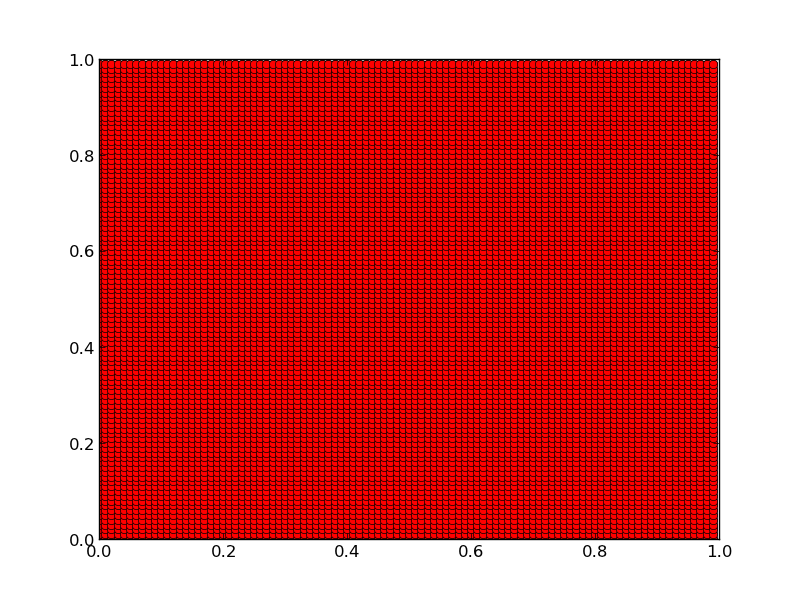
\includegraphics[scale=0.25]{0classregions.png}
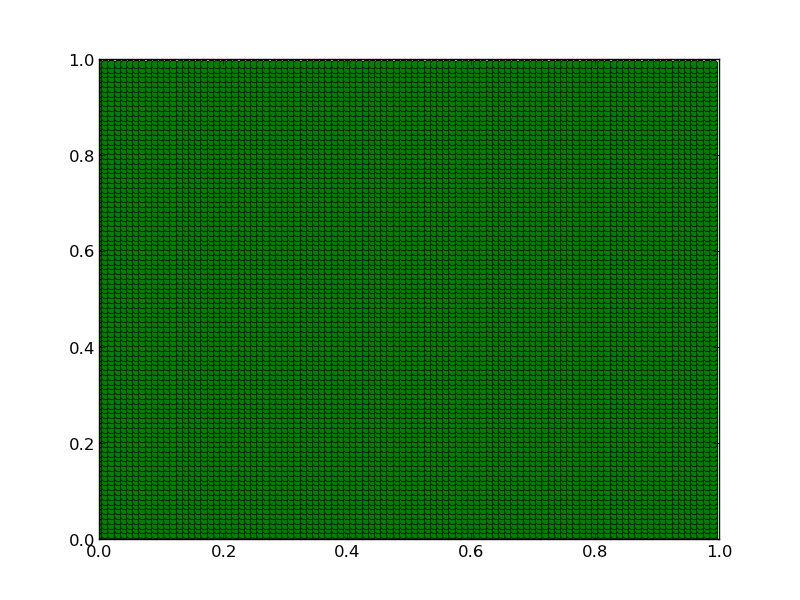
\includegraphics[scale=0.25]{10classregions.png}
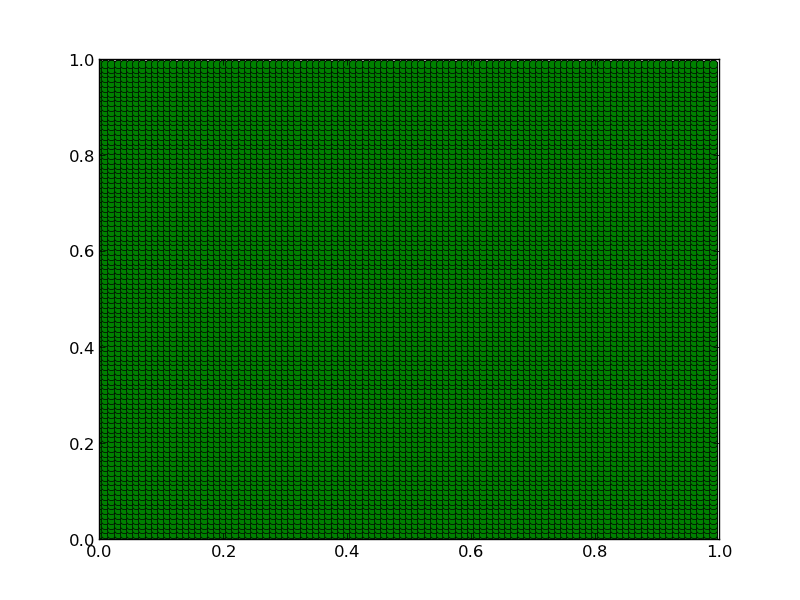
\includegraphics[scale=0.25]{100classregions.png}\\
\hspace{100px}1000 Epochs \hspace{120px}10000 Epochs\\
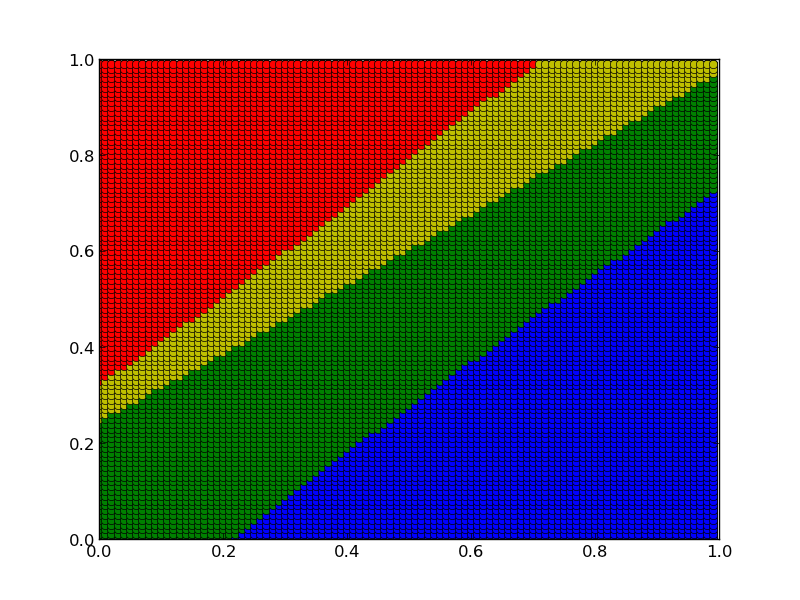
\includegraphics[scale=0.25]{1000classregions.png}
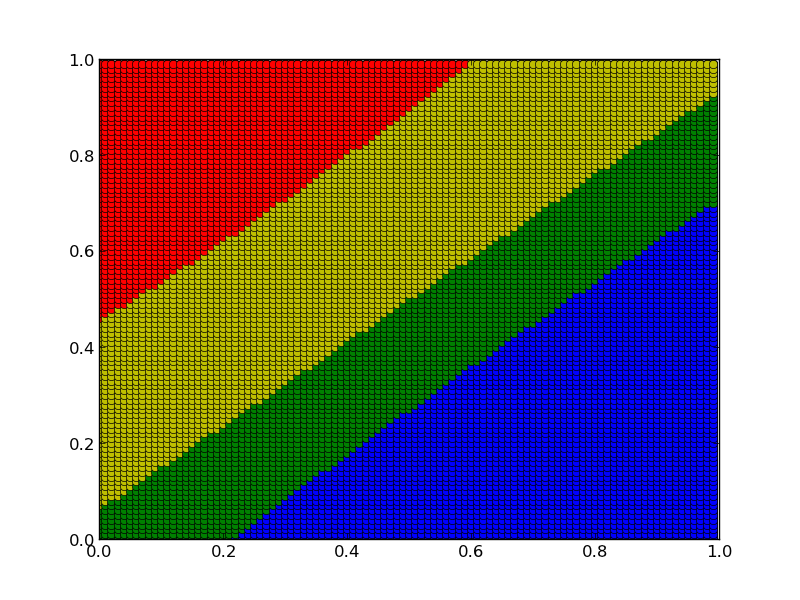
\includegraphics[scale=0.25]{10000classregions.png}

\subsection*{Errors}
\hspace{50px}X:  Number Wrong Y: Epochs \hspace{170px} SSE vs Epochs\\
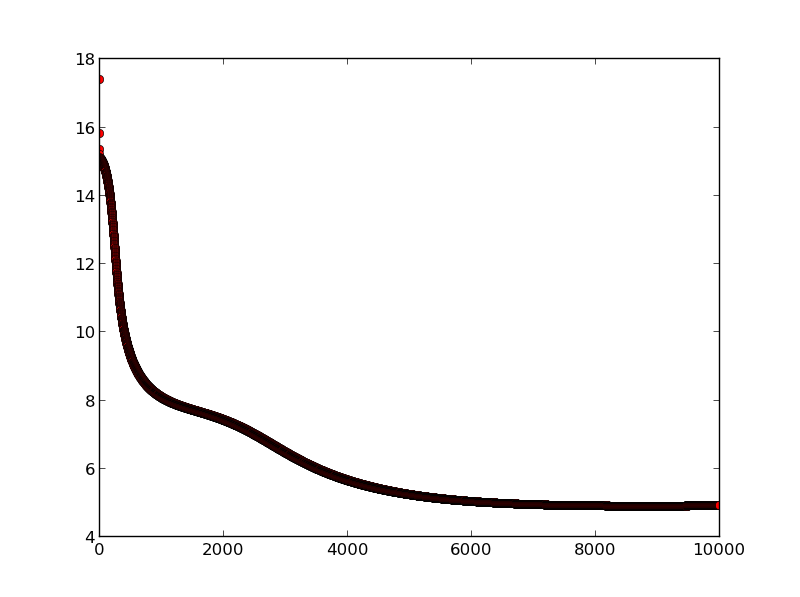
\includegraphics[scale=0.45]{10000iters.png}
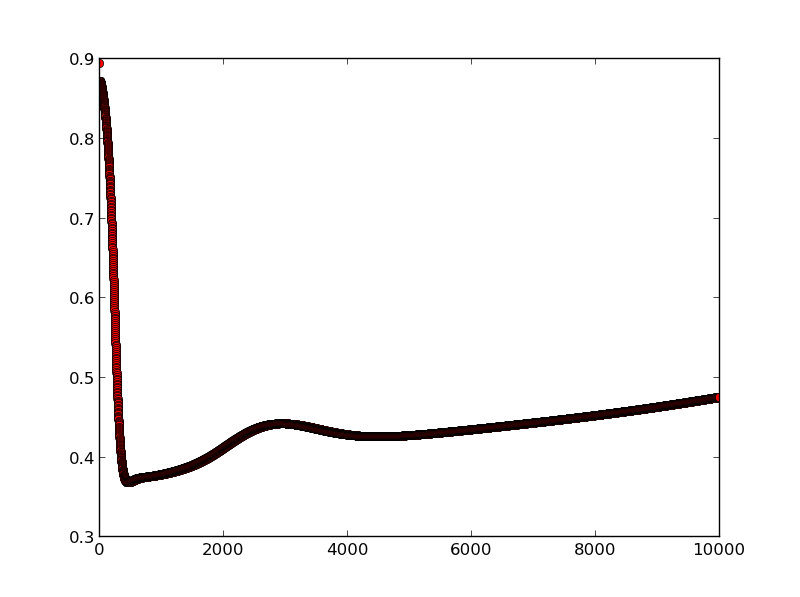
\includegraphics[scale=0.45]{error.png}

\section*{Discussion}
\indent  My best result was either 10,000 epochs depending on the run and metric used. They both had roughly the same results but different errors.  This is what I predicted.  As I noted above I didn't think my network would overfit the data too much, and it didn't.  As you can see from the above error data, I had a steady decrease barring some noise in the beginning then a slight increases.  The classification regions really shaped up nicely as time went on.  At first it was mostly one color, but by 1000 epochs definite regions had formed.  By 10000 epochs those regions had become more well defined and accurate.  Additionally, even though the regions didn't shift that much the error consistently rose a little.  The learning curve was about as expected considering the results.  There was some noise, but it became more accurate as time passed.  Randomness also unsurprisingly played a large factor into my results.  Even after 10,000 epochs I had a lot of variance in accuracy.  I had times where I was down around 50 percent after that long and I had times where I hit 85 percent after a few hundred.  \\
\indent I liked this assignment a lot.  I implemented my network very generically.  I can construct it with any architecture I wanted (I enjoyed playing around with different numbers of nodes) and assign any activation function to my nodes.  I think I'm most of the way to a framework and I'll probably continue to work with this after this project is done.  I also liked the practical part of the assignment.  It very much felt like a real world problem, and the fact that the training data was so noisy contributed to the realness aspect for me.  All in all, I really enjoyed this project.  
\end{document}